\documentclass[]{article}

\usepackage{fancyhdr}
 \pagestyle{fancy}
\rhead{\textsc{Scott O`Connor}}

\usepackage{lmodern}
\usepackage{amssymb,amsmath}
\usepackage{ifxetex,ifluatex}
\usepackage{fixltx2e} % provides \textsubscript
\ifnum 0\ifxetex 1\fi\ifluatex 1\fi=0 % if pdftex
  \usepackage[T1]{fontenc}
  \usepackage[utf8]{inputenc}
\else % if luatex or xelatex
  \ifxetex
    \usepackage{mathspec}
    \usepackage{xltxtra,xunicode}
  \else
    \usepackage{fontspec}
  \fi
  \defaultfontfeatures{Mapping=tex-text,Scale=MatchLowercase}
  \newcommand{\euro}{€}
\fi
% use upquote if available, for straight quotes in verbatim environments
\IfFileExists{upquote.sty}{\usepackage{upquote}}{}
% use microtype if available
\IfFileExists{microtype.sty}{%
\usepackage{microtype}
\UseMicrotypeSet[protrusion]{basicmath} % disable protrusion for tt fonts
}{}
\ifxetex
  \usepackage[setpagesize=false, % page size defined by xetex
              unicode=false, % unicode breaks when used with xetex
              xetex]{hyperref}
\else
  \usepackage[unicode=true]{hyperref}
\fi
\usepackage[usenames,dvipsnames]{color}
\hypersetup{breaklinks=true,
            bookmarks=true,
            pdfauthor={},
            pdftitle={The Meaning of Life 2},
            colorlinks=true,
            citecolor=blue,
            urlcolor=blue,
            linkcolor=magenta,
            pdfborder={0 0 0}}
\urlstyle{same}  % don't use monospace font for urls
\usepackage{graphicx,grffile}
\makeatletter
\def\maxwidth{\ifdim\Gin@nat@width>\linewidth\linewidth\else\Gin@nat@width\fi}
\def\maxheight{\ifdim\Gin@nat@height>\textheight\textheight\else\Gin@nat@height\fi}
\makeatother
% Scale images if necessary, so that they will not overflow the page
% margins by default, and it is still possible to overwrite the defaults
% using explicit options in \includegraphics[width, height, ...]{}
\setkeys{Gin}{width=\maxwidth,height=\maxheight,keepaspectratio}
\setlength{\parindent}{0pt}
\setlength{\parskip}{6pt plus 2pt minus 1pt}
\setlength{\emergencystretch}{3em}  % prevent overfull lines
\providecommand{\tightlist}{%
  \setlength{\itemsep}{0pt}\setlength{\parskip}{0pt}}
\setcounter{secnumdepth}{0}

\title{The Meaning of Life 2}
\author{Scott O’Connor}


% Redefines (sub)paragraphs to behave more like sections
\ifx\paragraph\undefined\else
\let\oldparagraph\paragraph
\renewcommand{\paragraph}[1]{\oldparagraph{#1}\mbox{}}
\fi
\ifx\subparagraph\undefined\else
\let\oldsubparagraph\subparagraph
\renewcommand{\subparagraph}[1]{\oldsubparagraph{#1}\mbox{}}
\fi

\begin{document}
\maketitle

\subsection{Introduction}\label{introduction}

Recall Tolstoy's question:

\begin{quote}
\ldots{} My question - that which at the age of fifty brought me to the
verge of suicide - was the simplest of questions, lying in the soul of
every man from the foolish child to the wisest elder: it was a question
without an answer to which one cannot live, as I had found by
experience. It was: ``What will come of what I am doing today or shall
do tomorrow? What will come of my whole life?'' (Tolstoy, p.14)\footnote{Tolstoy, Leo, \href{/Teaching/Examined/Meaning/Tolstoy.pdf}{`A
  Confession'}, 1882}
\end{quote}

\begin{quote}
Differently expressed, the question is: ``Why should I live, why wish
for anything, or do anything?'' It can also be expressed thus: ``Is
there any meaning in my life that the inevitable death awaiting me does
not destroy? (Tolstoy, p.14)
\end{quote}

Life has meaning only if it has significant value or purpose over time,
where this value makes life choice worthy. There are two different ways
of understanding this value:

\begin{itemize}
\item
  \textbf{Internal Value:} the value or purpose that comes when people
  see their goals or purposes as inherently valuable or worthwhile.
\item
  \textbf{External Value:} Meaning or purpose that comes from outside of
  ourselves in relationship to something that we may or may not be aware
  of.
\end{itemize}

When we ask about the meaning of life, we are asking about internal
value. We are asking why we should feel that there is something in our
lives that makes them worthwhile. Is there any project or goal that
could shape our psychology so dramatically that we are motivated to get up in the morning, keep going,
and find all the trials and tribulations of life worthwhile? Pessimists, recall, claim that no. Their
argument:

\begin{enumerate}
\def\labelenumi{\arabic{enumi}.}
\tightlist
\item
  Life is choice worthy only if it has internal value.
\item
  Life has internal value only if life has external value.
\item
  Life has no external value.
\item
  Life has no internal value (from 1--3).
\item
  Life is not choice worthy (from 1 \& 4).
\end{enumerate}

We saw that Tolstoy argues for Premise 2 and 3 by way of a fable:

\begin{figure}[htbp]
\centering
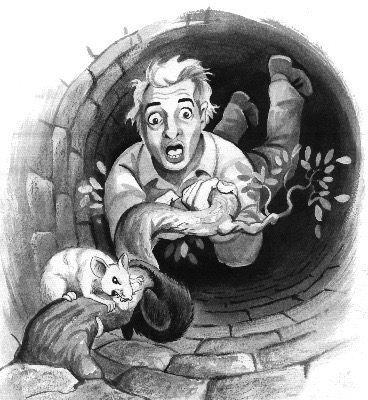
\includegraphics{Tolstoy.jpg}
\caption{The sweetness of life?}
\end{figure}

This argument is valid; the conclusion follows form the premises. Is it
sound, i.e., are the premises true? Optimists argue not. There are two
versions of Optimism. The first version accepts Premises 1 and 2, but
rejects Premise 3. They find external value in religion. The second type
of Optimist accepts Premise 3, that life has no external value, but
denies that internal value depends on there being external value, i.e.,
they deny Premise 2. The first type of Optimism is associated with
Theism, the second with Atheism. I discuss each in turn.

\subsection{Theism}\label{theism}

Tolstoy did not remain depressed. He reports meeting and talking with
rural farmers at a time in Russia when farmers lived a menial existence.
They had nothing. Yet Tolstoy sees in these rural farmers an acceptance
of life's vicissitudes. Reclaiming his faith, he realized that he had
found value in the wrong things. His art, his family, etc., could never
provide the meaning he had sought. But God, an eternally perfect being,
could provide that value. Tolstoy comes to accept the following two
claims:

\begin{enumerate}
\def\labelenumi{\arabic{enumi}.}
\item
  A human's life has external meaning only because it is part of God's
  plan, a grand cosmic order that encompasses every entity in the
  universe.
\item
  A human's life can have internal meaning if they align their
  life---their goals, projects, ambitions---with God's plan.
\end{enumerate}

On this view, life will be choice worthy if you can identify God's plan
for you and set about realizing that plan.

\subsection{Meaning \& Christianity}\label{meaning-christianity}

Tolstoy doesn't detail how Christianity construes the meaning of life.
He merely says that if you believe that God exists, then you can see
that your life has some external value. But can we say something more
about what this external value consists in?

At this point, Christians point to one person, Jesus, who they claim had
a meaningful life. Christians can claim that Jesus's life shows us that
God cares about human lives; Jesus was sent to save mankind. Reflecting
on the details of his life, we can also construe the internal and
external value of Jesus's life as follows:

\textbf{Prime Example:} His life had a purpose. All of Jesus' life
involves suffering for the sake of man kind. Saving mankind is the
external value his life had. All the aspects of his life were organized
around this one overarching purpose; he thought his life had God given
external purpose and spent his time and energy trying to fulfill that
purpose.

Christians also emphasizes other characters with God given purposes.
Noah, the Saints, the Apostles, are all individuals who were supposedly
given important jobs by God. These tasks, these jobs, give their life
external value according to Christianity. Their lives also had internal
value because they identified their God given purposes, saw them as
worthwhile, and devoted their time and energy to realizing them.

\subsection{Objection}\label{objection}

Here I briefly raise a problem for this account of the meaning of life.
Suppose we grant that the lives of Jesus, Noah, the other Saints had
external value because each of them had a God given purpose. It does not
thereby follow that each human has a God given purpose. The candidates
for this God given purpose seem unsatisfactory:

\textbf{Suggestions 1:} Our purpose is to serve God. This is a very
natural suggestion. A Theist might claim that we were created by God to
do his will. That would seem to give our lives the significance we
desired. The problem, though, is that being in service to someone is not
obviously a thing we would always choose. Granted, if God created us to
serve him, then our lives would be significant to God. But notice that
bees are significant to the bee keeper, yet that hardly shows us why a
bee should find its own life significant.

To motivate this objection, consider the very far fetched idea that God
created us to perform a very specific role. Once our species has grown
large enough, he will signal to an alien race to move to Earth where
they will find a new rich food source. Us! If this were the case, God
would have crated us to be the food in some alien's hamburger. We would
have a role in his grand design. We would even know what it is. I doubt,
though, that anyone would be happy to find out that they were created as
food for some superior being. A menial role in a stage designed for
another does not make life choice worthy.

There is a second worry with the claim that God created us to serve him.
God is all loving, all knowing, and all powerful. If he is all loving,
he would never have created us merely to serve him, especially since our
lives involve so much suffering and pain. Suppose that we had the
ability to create a a new fully conscious species. It is only an evil
creator that would create such beings to suffer and toil in servitude to
them.

\textbf{Suggestion 2:} The existence of God shows that we have a
purpose. He is all loving, therefore he would never have created us
without a purpose. However, since he is all loving, he would never have
created us merely to serve him. Nevertheless, we do not know why he
created us, to what end he intended our lives to serve.

This also seems a natural suggestion. The idea is that we do have a
purpose, but we just do not know what it is. The problem is that the
suggestion avoids answering the question at hand. How, if at all, would
the existence of God provide life with external meaning?

By themselves, these objections do not completely undermine the Theist's
account of the meaning of life. What they do, however, is show that
belief in God should not in itself be comforting. For God's existence to
be comforting, we need to know why he created us, to what end our lives
serve. Unless those details are forthcoming, the unsettling possibility
is left open that he created us for reasons that none of us should be
happy to live with.

\subsection{Atheism}\label{atheism}

Our second optimistic approach to the meaning of life rejects the need
for external value altogether. These optimists ask us to consider the
lives of people who clearly lead meaningful lives. If we can identify
why we think those lives valuable, we might be able to decide how, we
ourselves, can live meaningful lives without external value.

Who has lived a meaningful life? M.L.K, Gandhi, Einstein, Leonardo Di
Vinci are clear candidates. Can we see anything similar to their lives?

\begin{enumerate}
\def\labelenumi{\arabic{enumi}.}
\tightlist
\item
  Life had some dominant, over-all goal which gave direction to a great
  many of the individual's actions.
\item
  Actions were performed with a special zest that was not present before
  the person became attached to his goal or would not have been present
  if that person had no such goal.
\end{enumerate}

\subsection{Further Considerations}\label{further-considerations}

Susan Wolf has identified another few key features to this Optimist
account by contrasting the meaningless life from the meaningful life:

\begin{enumerate}
\def\labelenumi{\arabic{enumi}.}
\tightlist
\item
  The meaningless
\end{enumerate}

Wolf wants to give an account of what it is that makes an individual
life meaningful.

\begin{itemize}
\item
  She begins by shooting down an alternate account. She doesn't think
  that a life is meaningful iff it satisfies a subjective criteria like
  making the person happy.
\item
  Paradigm cases of meaningful lives---Gandhi, Mother Teresa, and
  Einstein, for example are not particularly happy lives.
\item
  Additionally, paradigm cases of meaningless lives-The Blob, for
  example-are actually filled with a good amount of subjective happiness
  and contentedness.
\end{itemize}

\begin{description}
\tightlist
\item[Wolf's account:]
A meaningful life is one that is a) actively and at least somewhat b)
successfully engaged in a project (or projects) of c) positive value.
\end{description}

There are three cases clauses to this definition that require defense.

\subsection{Active vs.~Non-Active Life}\label{active-vs.non-active-life}

Consider the cases of people whose lives are useless due to a lack of
activity: The Blob and the idle rich. Such lives seems useless. Wolf
asks us to conclude, with her, that a meaningful life must be one
actively engaged in some project. These projects are any kind of ongoing
activity or involvement. The projects engage the person, they see them
as constituting part of what their life is about and they pursue them
with zest.

\subsection{Actively engaged in a wrong
project.}\label{actively-engaged-in-a-wrong-project.}

Consider cases in which a life, though actively engaged, is wasted on a
project without any positive value. Someone might decide to adopt as
their life project the task of counting the number of grains of sand on
Sandy Hook beach. Someone might decide to take as their project the task
of everyday digging a hole and re-filling it. These projects seems
worthless. A life devoted to them cannot be a meaningful one.

So a meaningful life must be one dedicated to project of some positive
value.

\subsection{Success vs.~non-Success}\label{success-vs.non-success}

Consider cases in which the project around which somebody has organized
their life is revealed to be bankrupt, e.g., the inventor who devotes
their life to creating an automated car only to be beaten to the punch
by Google. Or the author who devotes decades to writing the biography of
some figure only to see someone else beat them to it. Or the CEO who
spends a life developing a business that is superseded by new
technologies, e.g., the CEO of a nuclear power plant company that ends
up seeing nuclear power replaced by solar power.

These lives are clearly tragic. There's something miserable about
devoting your life to a project that never sees fruition. So, Wolf
claims, that the projects must be successful for our lives to be
meaningful.

\end{document}
